\documentclass{article}
\usepackage{tikz, comment}
\usepackage{pifont}
\usepackage{fontspec, pgfplots}
\usetikzlibrary{arrows, decorations.markings, decorations.pathreplacing}
\begin{comment}
:Title: Not defined yet
:Tags: adjugate, classical adjoint;end behavior;additive inverse of a matrix;nth partial sum;perimeter
:Prob: 0.3195;0.2764;0.26;0.2579;0.2537
:Author: Prof.Hu Ji-shan, HKUST
:Slug: No name yet

Description Here.........
\end{comment}
\begin{document}\centering 

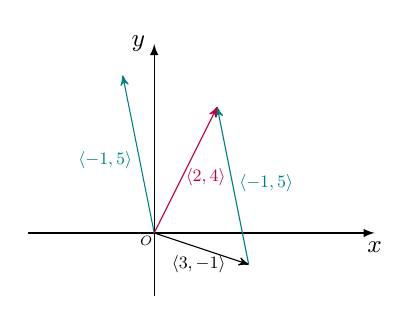
\begin{tikzpicture}[>=latex,xscale=.5*0.8, yscale=.5*0.8][font=\sf\small] 

%\draw[xstep=1cm,ystep=1cm,color=gray!80] (0, -1) grid (8, 8);

    	\foreach \x in {}
     		\draw (\x,2pt/8) -- (\x,-2pt/8)
			node[anchor=north] {\tiny$\x$}
			;

    	\foreach \x in {}
     		\draw (\x,2pt/1) -- (\x,-2pt/1)
			node[anchor=south] {\tiny$\x$}
			;
    	\foreach \y in {}
     		\draw (-2pt/1,\y) -- (2pt/1,\y)
			node[anchor=east] {\tiny $\y$}
			;

\draw[->] (-4, 0) -- (7, 0)node[below] {$x$} ;
\draw[->] (0, -2) -- (0, 6)node[left] {$y$} ;

\draw[->, >=stealth'] (0, 0)--(3, -1)node[black, below, midway, pos=0.5, xshift=-1, yshift=0, scale=0.7] {$\langle 3, -1 \rangle$};
\draw[teal, ->, >=stealth'] (0, 0)--(-1, 5)node[left, midway, pos=0.5, xshift=0, yshift=-2, scale=0.7] {$\langle -1, 5 \rangle$};

\draw[teal, ->, >=stealth'] (3, -1) -- (2, 4)node[right, midway, pos=0.5, xshift=0, yshift=1, scale=0.7]{$\langle -1, 5 \rangle$};

\draw[purple, ->, >=stealth'] (0,0) -- (2, 4)node[right, midway, pos=0.4, xshift=0, yshift=2, scale=0.7]{$\langle 2, 4 \rangle$};

\node[scale=0.7] at (-0.2/0.8, -0.2/0.8) {\scriptsize$O$};

\end{tikzpicture}
\end{document}